\section{Definition}

To facilitate illustration, we would define a set of notations which we will use throughout the whole paper: 

\begin{table}[h]
\centering
\begin{tabular}{ll}
\hline \hline
Notation      & Definition               \\ \hline
\textit{$D_L$}    & Labelled data            \\
\textit{$D_U$}    & Unlabelled data pool     \\
\textit{$D_B$} & Selected unlabelled data \\
\textit{I}    & Informativeness          \\ 
\textit{$M_T$}    & Task learner             \\
\textit{Q}    & Query strategy     \\
\textit{$x$} & Data instance \\
\textit{$y$} & Data label \\
\hline
\hline
\end{tabular}
\end{table}

We describe the typical framework as follows: A complete active learning framework consists of several key components: Data, Learner, Query strategy and Oracle. 
There two types of data: labelled data (minority portion) and unlabelled data (majority portion). 
First, $M_T$ is initialized with $D_L$. After that, $Q$ will select the most informative samples from $D_U$ depending on the predictions from current $M_T$. The selected $D_B$ are sent to oracle for labour to label. Next, the data-label pairs are feedback to $M_T$ for further model evolution. Query and learner evolution would be iterated until labelling budget is exhausted or learner performance has converged.  

\begin{figure}[h!]
    \centering
    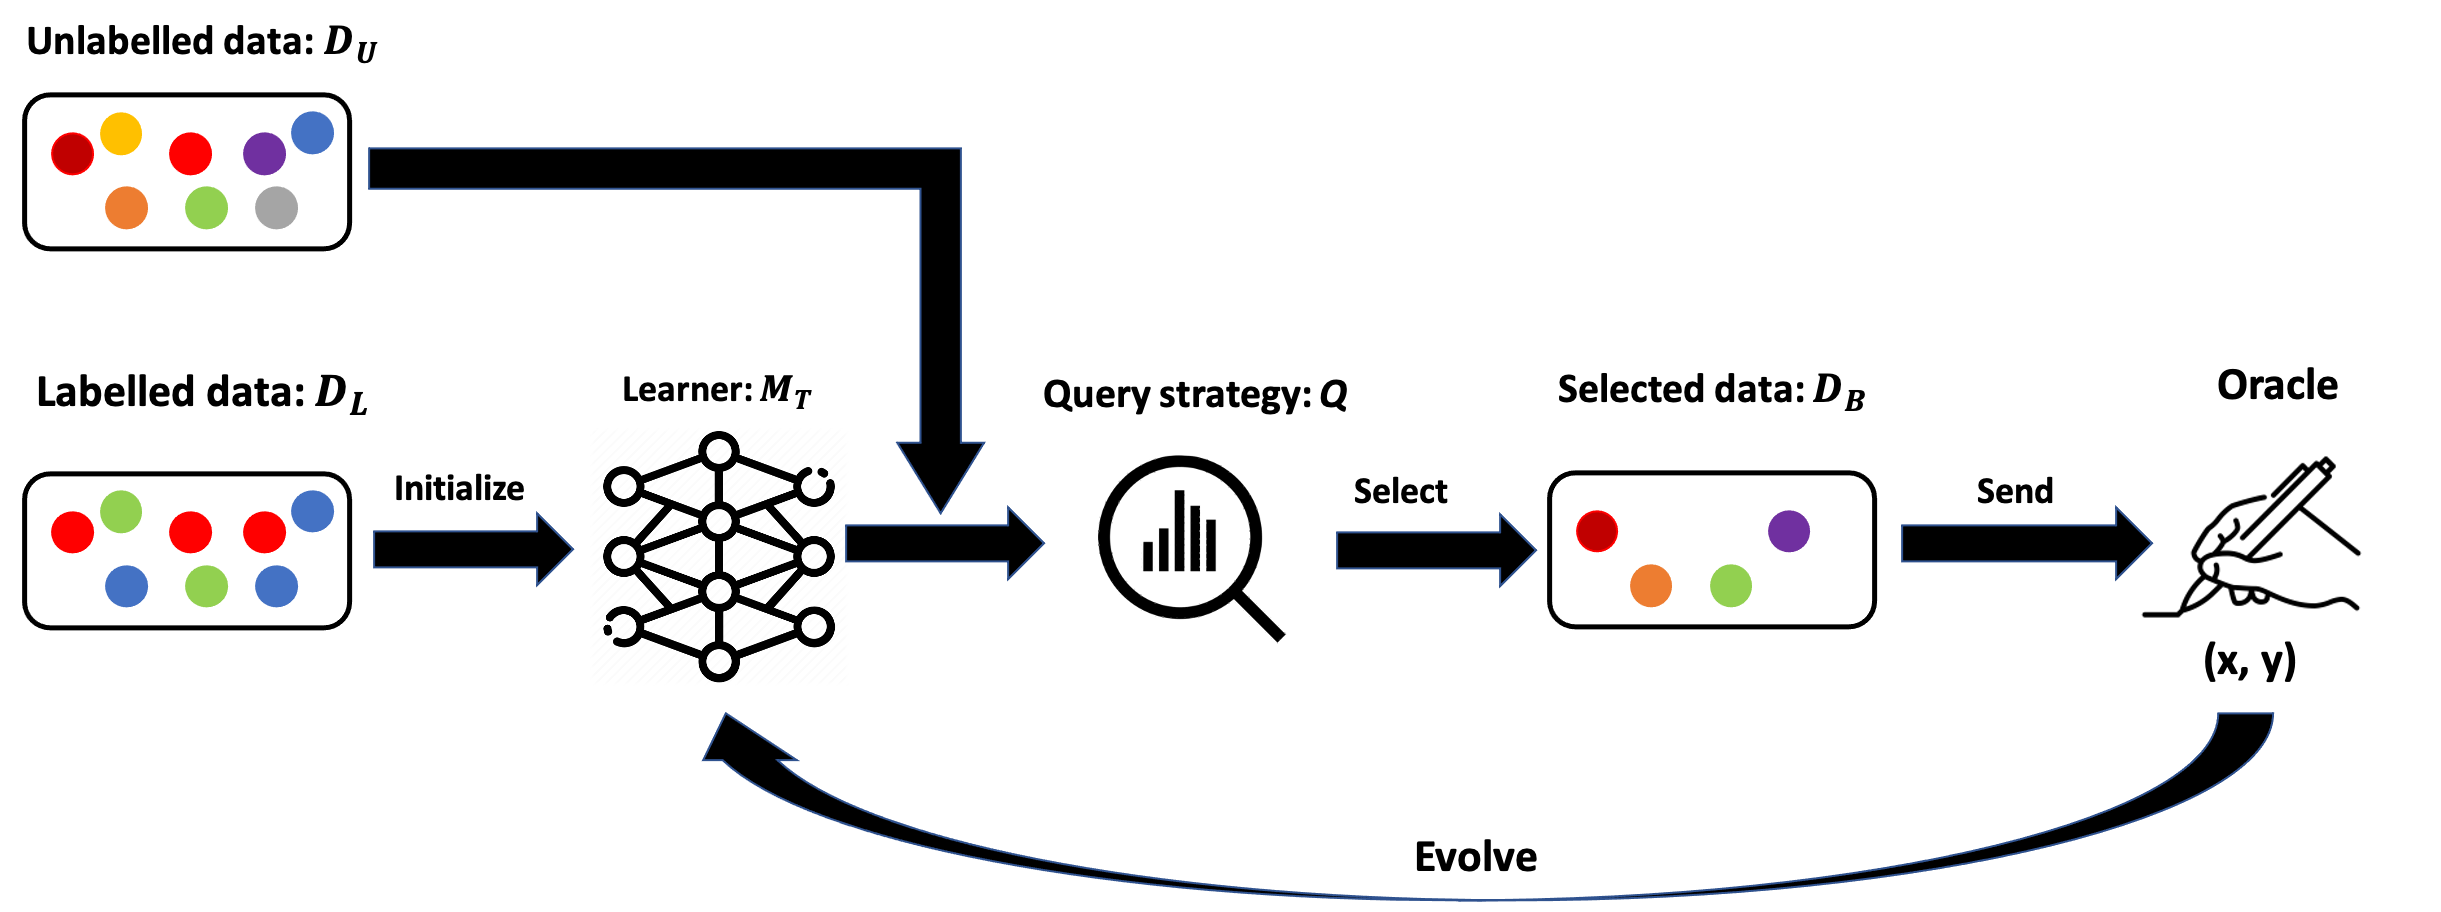
\includegraphics[width=\textwidth]{images/al_framework.png}
    \caption{AL framework}
    \label{fig:framework}
\end{figure}

